\documentclass[tikz,border=5pt]{standalone}
\usetikzlibrary{positioning}

\tikzset{
    block/.style = {draw, thick, rectangle},
    >=latex,
    font=\footnotesize,
    align=center,
    fonttitle/.style={fill=white,rectangle,text width=4em,inner sep=1pt,font=\bfseries\small},
    fontlabel/.style={font=\footnotesize},
    fontreward/.style={fill=white,font=\footnotesize}}
    
\begin{document}
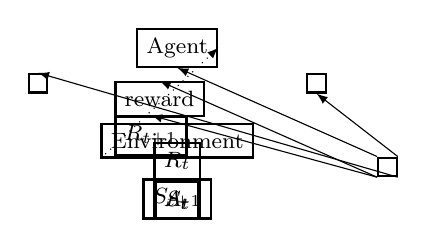
\begin{tikzpicture}[node distance=.7cm]
    %Environment
    \node[block](env){Environment};
    \node[above=of env,block](agent){Agent};
    \node[block,anchor=north east,xshift=2.8cm,yshift=-0.2cm](agt-env){};
    %Reward
    \node[block,anchor=south west,yshift=0.3cm,xshift=-0.8cm](reward){reward};
    \node[block,anchor=south west,yshift=-0.2cm,xshift=-0.8cm](rewardprime){$R_{t+1}$};
    %State
    \node[block,anchor=south west,yshift=0.6cm,xshift=-1.9cm](state){};
    %Actions
    \node[block,anchor=south east,yshift=0.6cm,xshift=1.9cm](action){};
    %Transition
    \draw[->](agt-env.north west)--(agent.south);
    \draw[->](agt-env.south west)--(reward.north);
    \draw[->](agt-env.south west)--(rewardprime.north);
    \draw[->](agt-env.south east)--(state.north);
    \draw[->](agt-env.north east)--(action.south);
    %Labels
    \node[block,anchor=south,yshift=-1cm](slabel){$S_t$};
    \node[block,anchor=south,yshift=-1cm](alabel){$A_t$};
    \node[block,anchor=south,yshift=-0.5cm](rlabel){$R_t$};
    \node[block,anchor=south,yshift=-1cm](slableft){$S_{t+1}$};
    %Connection
    \draw[->,dotted](env.south west)--(agent.east);
\end{tikzpicture}
\end{document}